% !TEX root = main.tex
% NullSpace

\section{ Null Space }%
Null space contains all special solutions. How many special solutions?
One for every free variable.


Augmented matrix


有解的条件: the condition for solvability

So I can \textbf{proceed} to so

Solvability condition on b
\( Ax = b \) is solvable when \( b \) is in \( C(A) \)
\( b \) has to be a combination of the columns
If a comb of rows of A gives zero \textbf{row}, the same comb of rows of b gives zero.

They are both equivalent to the solvability of the system

To find complete solution to \( Ax = b \)
\begin{enumerate}
	\item \( x_\text{particular} \): Set the free variables to zero. It's ``free''.
\end{enumerate}


\begin{listing}
	\begin{minted}[linenos,numbersep=5pt,frame=lines,framesep=2mm]{matlab}
A = [ 1 2 2 2 1; 0 0 2 4 3 ];
b = [1;3];
AA = [A b; zeros(1,length(A)+1)]
length(AA)
R=rref(AA);
\end{minted}
	\caption{matlab code}
	\label{lst:matlab_code}
\end{listing}

What's free variable?
\( \implies a \to b \)
Reduce row echelon form

\begin{equation*}
	A (x_p + x_n) = b
\end{equation*}

Free variables = \( n -r \). If \( n = r \), there is no free variable.
\(  N(A) = { \text{zero vector} } \)

\subsection{\( r = n \)}%
There is a unique solution.

\subsection{\( r = m \)}%
Since \( r = m \), I can solve \( Ax = b \) for every \( b \).

\subsection{\( r = m = n \)}%
Equivalence:
\begin{itemize}
	\item reversible
	\item \( r = m = n \)
	\item \( \rref(A) = I \)
	\item Both null space \( N(A) \) and left null space \( N(A\Tr) \) only contain zero vector
\end{itemize}

Unique solution if it exists
\subsection{\( r = n < m \)}%
\begin{equation*}
	R =
	\begin{bmatrix}
		I \\ O
	\end{bmatrix}
\end{equation*}

0 or 1 solution, because there is no free variable.
Where there is no free variable, there is no solution except zero vector in null space.
And there is no coefficient \(c\) for \( c \vb{x}_{p} \).
The complete solution is merely the unique particular solution.
Or \(\vb{x} = \vb{x}_p + \vb{x}_n \qq{where} \vb{x}_n = 0 \).

\subsection{\( r = m <n \)}%

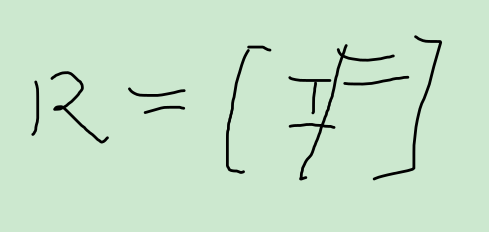
\includegraphics[width=0.3\textwidth]{figures/2021-09-17T190337+0800.png}
rather than
\(
R =
\begin{bmatrix}
	I & F
\end{bmatrix}
\)

There exists solutions. The number of equations \(>\) the number of unknowns.

\( \infty \) solutions.

We always have null space to deal with.

If we set all free variables to \(0\), the unique solution exists.

\subsection{\( r < m, r < n  \)}%
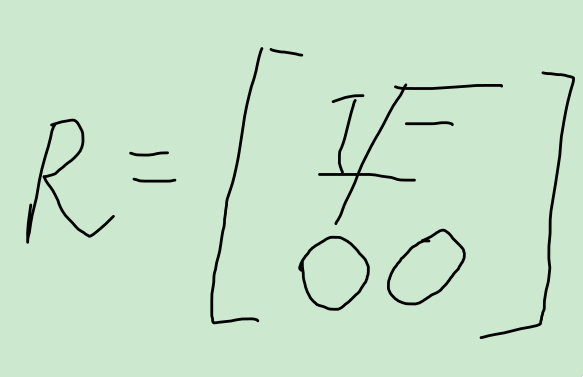
\includegraphics[width=0.3\textwidth]{figures/2021-09-17T191029+0800.png}

0 or \( \infty \) solutions

\begin{remark}
	The rank tells you everything about the number of solutions
\end{remark}

%%% vim: set ts=2 sts=2 sw=2 isk+=\: et cc=+1 formatoptions+=mM:
